\begin{figure}
    \begin{center}
    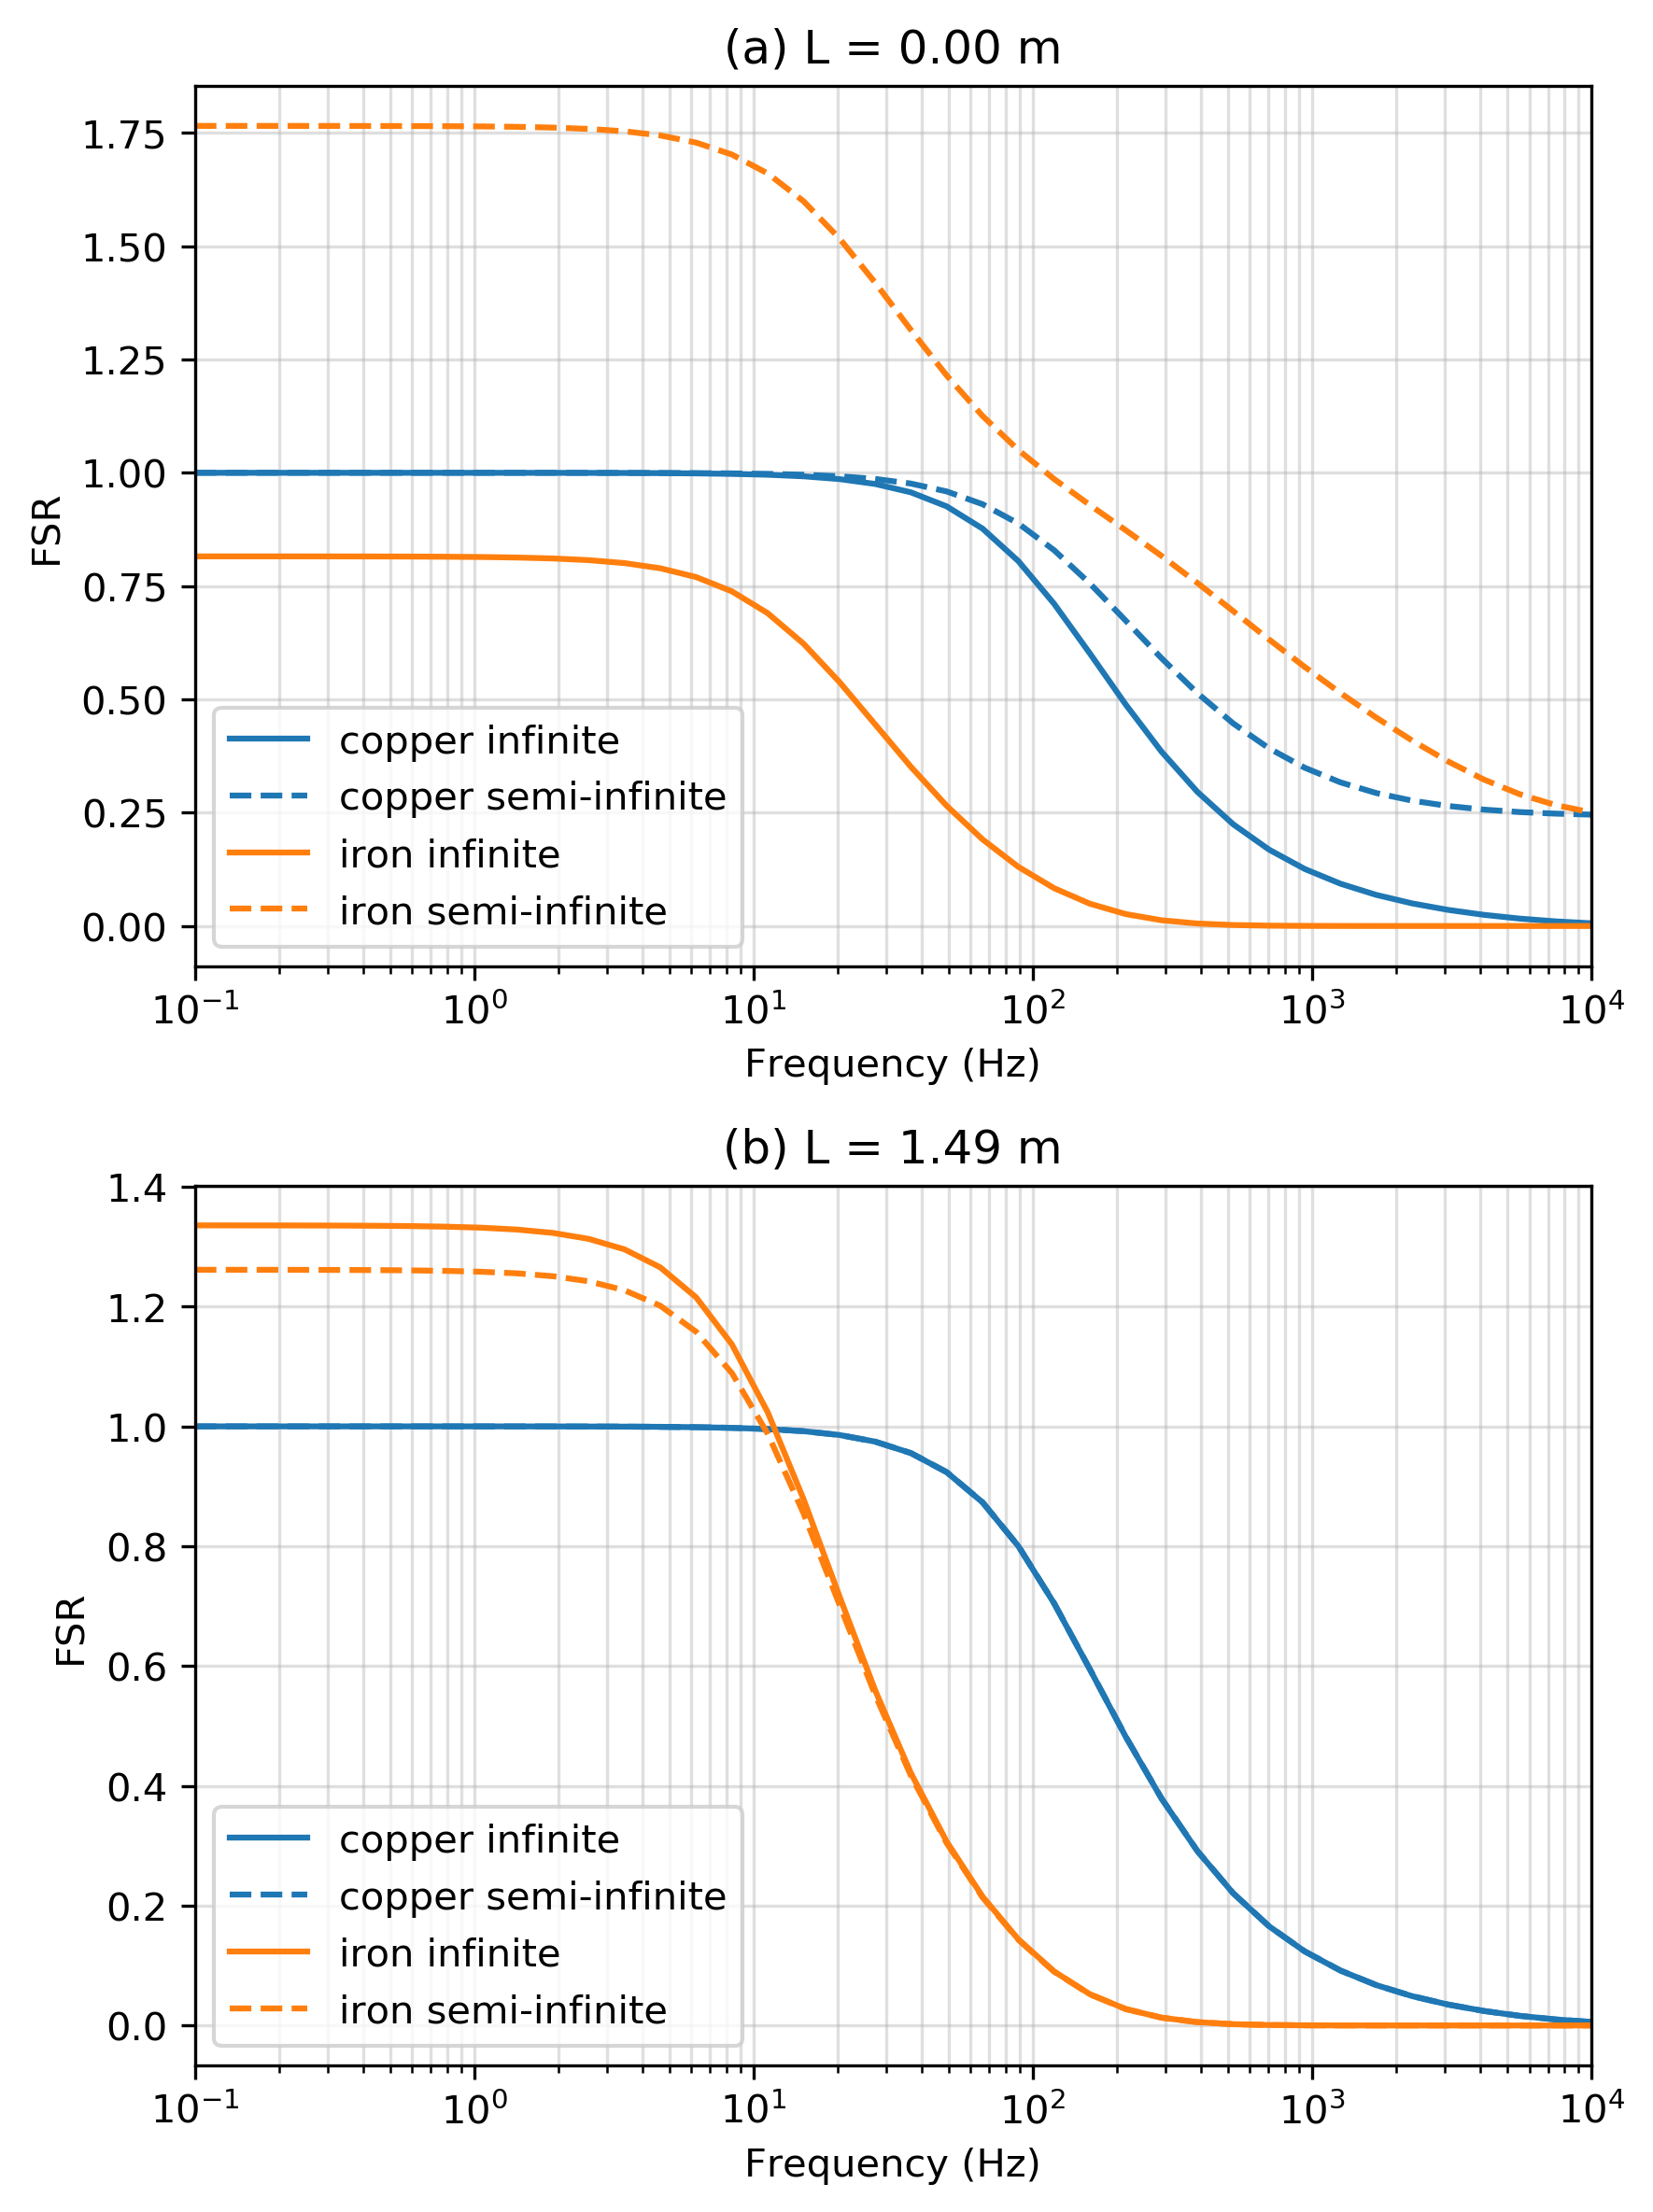
\includegraphics[width=0.6\columnwidth]{figures/casing_software/AugustinFSR.png}
    \end{center}
\caption{
    Field strength ratio (FSR), the ratio of the measured vertical magnetic field with the free space magnetic field, as a function of frequency for two different receiver locations.
    In (a), the receiver is in the same plane as the source, in (b), the receiver is 1.49 m offset from the source.
}
\label{fig:AugustinFSR}
\end{figure}
